%\documentclass[11pt]{article}  % for e-submission to ApJ
\documentclass[11pt]{NSF}  % for e-submission to ApJ

%\documentclass[12pt,preprint2]{aastex}  % for e-submission to ApJ - two column

%\documentclass[manuscript]{emulateapj}  % this makes everything look like ApJ

\usepackage{graphicx, natbib, color, bm, amsmath, epsfig}

%paper commands, for when not using aastex
\newcommand\physrep{Phys.~Rep.}
\newcommand\fcp{Fund.~Cosmic~Phys.}
\newcommand{\pre}{Phys Rev E}
\newcommand{\apj}{ApJ}
\newcommand{\apjs}{ApJS}
\newcommand{\aj}{AJ}
\newcommand{\aap}{A\&A}
\newcommand{\mnras}{MNRAS}
\newcommand{\araa}{ARA\&A}
\newcommand{\procspie}{Proc.SPIE}
\newcommand{\pasj}{PASJ}
\newcommand{\iaucirc}{IAU Circ.}
\newcommand{\aplett}{AP Letters}
\newcommand{\aaps}{AAPS}
\newcommand{\aapr}{AAPR}
\newcommand{\nat}{Nature}
\newcommand{\apjsupp}{ApJS}
\newcommand{\pasp}{PASP}
\newcommand{\apjl}{ApJL}
\newcommand\prl{Phys.~Rev.~Lett.}
\newcommand\apss{Ap\&SS}




%%%% PUT NEW COMMANDS AND DEFINITIONS HERE %%%%
\usepackage{graphicx, natbib, color, bm, amsmath, epsfig}

%
% Hijacked and hacked from aastex.cls
%
%\def\newblock{\hskip .11em\@plus.33em\@minus.07em}%

%\newcommand\plotone[1]{%
% \typeout{Plotone included the file #1}
% \centering
% \leavevmode
% \includegraphics[width={\eps@scaling\columnwidth}]{#1}%
%}
%\newcommand\plotone[1]{
% \includegraphics[width=3.0in]{#1}%
%}
%\let\tableline=\hline
%enzo commands
\newcommand\jcompphys{J.~Comput.~Phys}
\newcommand\physfluidsa{Phys.~Fluids~A}
\newcommand\physfluids{Phys.~Fluids}
\newcommand\physlettA{Phys.~Lett.~A}
\newcommand\jfm{J.~Fluid~Mech.}
\newcommand\ccm{Comput.~Phys.~Commun.}
\newcommand\jphysique{J.~Physique~I}
\newcommand\revmodphys{Rev.~Mod.~Phys.~}

%\newcommand\aap{\ref@jnl{A\&A}}% 
%\newcommand\prb{\ref@jnl{Phys.~Rev.~B}}% 
          % Physical Review B: Solid State 


\newcommand{\ratio}{\mathcal{R}}
\newcommand{\yt}{{\tt yt}}
\newcommand{\Lmax}{\ell_{\rm max}}
\newcommand{\enzo}{{\small Enzo}}
\newcommand{\menzo}{{EnzoMHD}}
\newcommand{\Menzo}{{EnzoMHD}}
\newcommand{\zeus}{{\small ZEUS}}
\newcommand{\Lbox}{L_{\rm box}}
\newcommand{\Nroot}{N_{\rm root}}
\newcommand{\K}{\,\rm K}
\newcommand{\dave}{DaveThena}
\newcommand{\grid}{{\tt grid}}

%\newcommand{\lct}[3]{\ensuremath{\epsilon_{#1,#2,#3}}}
\newcommand{\lct}[1]{\ensuremath{\epsilon_{#1}}}
%grid location commands.
\newcommand{\iph}{i + \frac{1}{2}}
\newcommand{\imh}{i - \frac{1}{2}}
\newcommand{\jph}{j + \frac{1}{2}}
\newcommand{\jmh}{j - \frac{1}{2}}
\newcommand{\kph}{k + \frac{1}{2}}
\newcommand{\kmh}{k - \frac{1}{2}}

\newcommand{\ipmh}{i \pm \frac{1}{2}}
\newcommand{\half}{\frac{1}{2}}
\newcommand{\quart}{\frac{1}{4}}
\newcommand{\tquart}{\frac{3}{4}}

%physics commands
\newcommand{\avir}{\ensuremath{\alpha_{\rm{vir}}}}
\newcommand{\mach}{\ensuremath{\mathcal{M}}}
\newcommand{\hmag}{\ensuremath{H_{\rm{M}}}}
\newcommand{\alfmach}{\ensuremath{\mathcal{M_{\rm{A}}}}}
%\newcommand{\msun}{\ensuremath{\rm{M}_\odot}}
\newcommand{\msun}{\ensuremath{M_\odot}}
\newcommand{\lsun}{\ensuremath{L_\odot}}
\newcommand{\rsun}{\ensuremath{R_\odot}}

\def\mch{\ensuremath{M_{\rm{Ch}}}}
\def\AD{{\rm{AD}}}

%math commands
\def\rms{\ensuremath{\rm{rms}}}
\newcommand{\pts}[1]{\emph{(#1 pts)}}
\newcommand{\dbd}[2]{\frac{ \partial #1 }{ \partial #2} }
\newcommand{\ddbd}[2]{\frac{ d #1 }{ d #2} }
\newcommand{\dDbD}[2]{\frac{ \mathrm{D} #1 }{ \mathrm{D} #2} }
\newcommand{\curl}{\nabla \times}
\newcommand{\divb}{\ensuremath{\nabla \cdot {\bvec}}}
\newcommand{\divv}{\ensuremath{\nabla \cdot {\vvec}}}
\newcommand{\divbo}{$\nabla \cdot {\bf B} = 0$}
\newcommand{\intd}[1]{\int_#1^{#1 + \Delta #1} }
\newcommand{\dt}{\Delta t}
\newcommand{\dx}{\Delta x}
\newcommand{\dy}{\Delta y}
\newcommand{\dz}{\Delta z}
\newcommand{\p}[1]{#1^\prime }
\newcommand{\pp}[1]{#1^{\prime \prime} }
\newcommand{\tff}{\ensuremath{t_{\rm{ff}}}}
\newcommand{\kkmin}{\ensuremath{k/k_{\rm{min}}}}
\newcommand{\kmax}{\ensuremath{k_{\rm{max}}}}

%dcc color commands
\definecolor{orange}{rgb}{1.        ,  0.54,  0}
\newcommand{\orange}[1]{\textcolor{orange}{#1}}

\newcommand{\gtt}[1]{\textcolor{green}{{\tt#1}}}
\newcommand{\red}[1]{\textcolor{red}{#1}}
\newcommand{\yellow}[1]{\textcolor{yellow}{#1}}
\newcommand{\blue}[1]{\textcolor{blue}{#1}}
\definecolor{meta}{rgb}{0.371,0.617,0.625} %cadet blue for
                                           %non-production worthy
                                           % discussion of the work
\newcommand{\meta}[1]{\textcolor{meta}{#1}}
\newcommand{\green}[1]{\textcolor{green}{#1}}
\newcommand{\aake}[1]{\textcolor{blue}{#1}}
\newcommand{\bld}[1]{\mathbf{#1}}

\def\here{\red{notes later}}
%\newcommand{\hilite}[1]{\textcolor{red}{#1}}
%\newcommand{\hilite}[1]{#1}

%\newcommand{\bold}[1]{{\bf #1}}
%the comment maker, dc: the first one will show all comments in green, 
%the second hides them all.
%\newcommand{\dc}[1]{\textcolor{green}{#1}}
\newcommand{\dc}[1]{}
%\newcommand{\dc}[1]{#1}
%\def\bvec{\ensuremath{\vec{B}}}
%\def\vvec{\ensuremath{\vec{v}}}
\def\Bvec{\ensuremath{{\bf B}}}
\def\Jvec{\ensuremath{{\bf J}}}
\def\Avec{\ensuremath{{\bf A}}}
\def\bvec{\ensuremath{{\bf b}}}
\def\vvec{\ensuremath{{\bf v}}}
\def\uvec{\ensuremath{{\bf u}}}
\def\rvec{\ensuremath{{\bf r}}}
\def\xvec{\ensuremath{{\bf x}}}
\def\kvec{\ensuremath{{\bf k}}}
\def\Omegavec{\ensuremath{{\bf \Omega}}}
\def\omegavec{\ensuremath{{\bf \omega}}}
%\newcommand{\BlockOut}[1]{}
\newcommand{\BlockOut}[1]{#1}
\newcommand{\imp}{\ensuremath{\implies}}
\newcommand{\question}[1]{\textcolor{red}{#1}}
\definecolor{pink}{rgb}{1.        ,  0.75294118,  0.79607843}
\definecolor{maroon}{rgb}{0.69019608,  0.18823529,  0.37647059}
\newcommand{\ToRead}[1]{\textcolor{maroon}{#1}}
\newcommand{\ToReadUrgent}[1]{\textcolor{red}{#1}}
\newcommand{\HaveRead}[1]{\textcolor{black}{#1}}
\newcommand{\Old}[1]{\textcolor{blue}{#1}}
\newcommand{\Scanned}[1]{\textcolor{meta}{#1}}
\newcommand{\dccnote}[1]{}
%\newcommand{\dccnote}[1]{\textcolor{red}{#1}}
\def\nn{\nonumber}

\newcommand{\get}[1]{\textcolor{red}{#1}}
\definecolor{gray}{rgb}{0.5,0.5,0.5}
\newcommand{\gray}[1]{\textcolor{gray}{#1}}
\newcommand{\clean}[1]{\textcolor{gray}{#1}}
\newcommand{\ToDo}[1]{\textcolor{red}{#1}}
\def\etal{{\sl et al.}}

%chemistry commands
\newcommand{\Htwo}{\ensuremath{\rm{H}_2}}
\newcommand{\twelveco}{\ensuremath{^{12}\rm{CO}}}
\newcommand{\thirteenco}{\ensuremath{^{13}\rm{CO}}}

\newcommand{\mhdlabel}{{_{MHD}}}
\newcommand{\gravlabel}{{_{Grav}}}
\newcommand{\fclabel}{{_{fc}}}
\newcommand{\explabel}{{_{exp}}}
\newcommand{\sci}[1]{\ensuremath{\times {10^{#1}}}}
\newcommand{\percc}{\ensuremath{\rm{cm}^{-3}}}
\newcommand{\gcc}{\ensuremath{\rm{g}\ \rm{cm}^{-3}}}
\newcommand{\kms}{\ensuremath{\rm{km}\ \rm{s}^{-1}}}
\newcommand{\cms}{\ensuremath{\rm{cm}\ \rm{s}^{-1}}}
\newcommand{\cmperg}{\ensuremath{\rm{cm}^{2}\ \rm{g}^{-1} }}
\newcommand{\cmcmpers}{\ensuremath{\rm{cm}^2\ \rm{s}^{-1} }}
\def\muG{\ensuremath{\mu\rm{G}}}
\def\micron{\ensuremath{\mu\rm{m}}}
\def\alf{Alfv\' en}
\def\Alfvenic{Alfv\' enic}
\def\sa{super-Alfv\' enic}
\def\Sa{Super-Alfv\' enic}
\def\suba{sub-Alfv\' enic}
\def\Suba{Sub-Alfv\' enic}
\def\transa{trans-Alfv\' enic}
\def\Transa{Trans-Alfv\' enic}
\def\cs{\ensuremath{c_{\rm{s}}}}
\def\va{\ensuremath{v_{\rm{A}}}}
\def\sfrff{\ensuremath{{\rm SFR_{ff}}}}
%\def\velocity{\ensuremath{\vec{v}}}
%\def\magnetic{\ensuremath{\vec{B}}}
\def\velocity{\ensuremath{{\bf v}}}
\def\magnetic{\ensuremath{{\bf B}}}
\newcommand{\Fourier}[1]{\ensuremath{\tilde{#1}}}
\def\hfw{0.49}
\def\hw{0.49}
\def\fw{0.9}

\def\ssp{\def\baselinestretch{1.0}\large\normalsize}

\def\rhoc{\ensuremath{\rho_{\rm{c}}}}
\def\erf{\ensuremath{\rm{erf}}}


\def\SUtotal{2.9\sci{5}       }%cut from table1.
\def\tfinal{T_{\rm{final}}}
\def\suzu{\ensuremath{\rm{SU}_{\rm{zu}}}}
\def\nzones{N_{\rm{z},\ell}}
\newcommand{\Lund}{\ensuremath{\mathrm{S}}}
%\newcommand{\SUestimate}[1]{\textcolor{red}{#1}}
\newcommand{\SUestimate}[1]{#1}
\def\SUtotal{1.6\sci{5}       }                                                       
%\def\SUturb{1.8\sci{4}}
%\def\SUcore{1.2\sci{4}}
%\def\SUcmb{2.6\sci{4}}
%\def\SUgal{2.2\sci{3}}
%\def\DiskTurb{5.6\sci{3} Gb}
%\def\DiskCore{1.6\sci{5} Gb}
%\def\Diskcmb{1.7\sci{4} Gb}
%\def\Diskgal{1.1\sci{4} Gb}
%\def\StoreTotal{1.9\sci{5} Gb}
\def\nameTurbulence{\emph{turbulence}}
\def\nameTurbShort{\emph{turb}}
\def\nameCores{\emph{cores}}
\def\nameCMB{\emph{foregrounds}}
\def\nameGalaxies{\emph{galaxies}}
\def\suPerZoneUpTurbulence{\ensuremath{2.0\sci{-11}}}
\def\suPerZoneUpCores{\ensuremath{6.2\sci{-11}}}
\def\suPerZoneUpCMB{\ensuremath{6.2\sci{-11}}}
\def\suPerZoneUpGalaxies{\ensuremath{3\sci{-10}}}

\citestyle{aa}  % correct formatting for ApJ style files

\usepackage{aas_macros}
\begin{document}

\begin{centering}
\begin{LARGE}
Scaling Information for 

``Four Projects in Astrophysical Magnetohydrodynamics''
\end{LARGE}

David Collins, PI

\end{centering}


\pagestyle{plain}

The four projects presented in this proposal will be using the code Enzo
\citep{Collins10, Bryan14}.
Enzo  is an open source adaptive mesh refinement (AMR) code that
has been used in hundreds of astrophysical works.  These studies include the
formation of the first stars \citep{Abel02}, clusters of galaxies \citep{Xu11}
and the large scale structure of the universe.  It employs several hydrodynamics
solvers, including the piecewise parabolic method  \citep[PPM,][]{Colella84}, two implementations of
magnetohydrodynamics (MHD), self-gravity, and Lagrangian particles that can be used
for collisionless dark matter, stars, dust, and passive tracers.  One of the
primary advantages of Enzo over other codes is its use of structured AMR, which
allows it to add resolution elements adaptively as dictated by the problem.  A
variety of refinement criterion are available.   The present studies will use
the divergence-preserving MHD module \citep{Collins10}.  For the patch solver we
use the
second order MHD method of \citet{Li08a} and the constrained transport method of
\citet{Gardiner05} to preserve the divergence-free constraint (\divbo) to
machine precision.  For the AMR, the divergence-free reconstruction of \citet{Balsara01}
is used to interface magnetic fields with the adaptive mesh.  For chemistry and
 thermodynamics used in the \nameGalaxies\ project, Grackle is used
\citep{Smith17}.  

To measure the behavior of the solvers, we ran a weak scaling test with the main
physics packages for the four projects.  The four projects are of two varieties:
the \nameCMB\ and \nameTurbulence\ projects employ driven turbulence and the
hydro/MHD solver, while the \nameCores\ and \nameGalaxies\ projects additionally
employ the gravity solver.  Thus we run two scaling studies, one with just the
MHD; and one with MHD, gravity, and AMR.  The For both studies,
a constant amount of
work, $128^3$ zones per task, was used for each node. 
Scaling was done from 8 through 4096
processors, with 64 threads per node (when possible).
For the AMR, one level covering 1/8 of the box by volume was used.
The packages in question do not depend heavily on the regime of
physics in question, so uniform gas was taken in each case.  The results can be
seen in Figure \ref{fig.scaling}.  Here we plot $\zeta = \frac{zone\
updates}{core\ second}$ vs. number of mpi tasks.
For ideal scaling, this will be independent of the number of processes.

The blue curve, applicable to the \nameCMB\ and \nameTurbulence\ suites, uses only the MHD
solver and random forcing.  This is extremely parallelizable, as the work is
entirely local.  The orange curve, applicable to the \nameCores\ and
\nameGalaxies\ projects,
uses the MHD solver, gravity solver, and AMR.  
The performance of this combination sharply declines at 512 threads.  
This is due to the gravity solver and AMR overhead.  

We use a value of $\zeta=10^5$ for the \nameCMB\ and \nameTurbulence\
simulations, and $7.4\sci{4}$ for the \nameCores\ and \nameGalaxies\
simulations to estimate the total cost for each suite of simulations.  We will
use 64 nodes for the first two, and 8 nodes for the second two.


\begin{figure} \begin{center}
    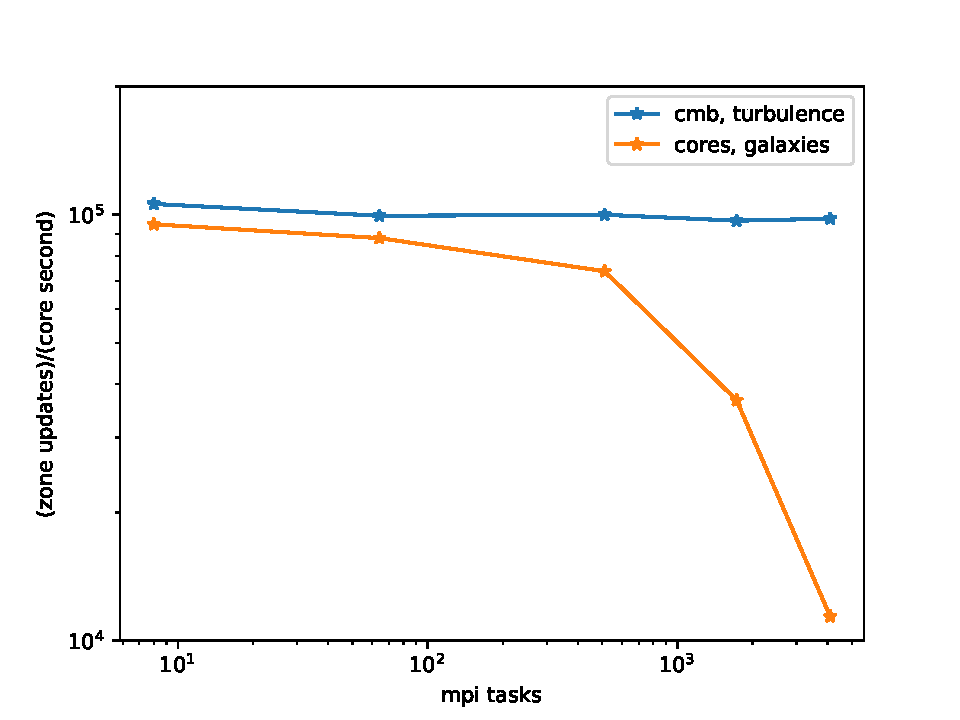
\includegraphics[width=0.99\textwidth]{figs/g49_zoneup.pdf}
\caption[ ]{Zone-pdates per core-second for weak scaling on
    Stampede 2.    
The blue curve only employs
    the MHD solver, in the configuration used for the \nameCMB\ and \nameTurbulence\
    simulations.  The orange curve employs the MHD solver as well as the gravity
    solver and AMR,
 and will be used for the \nameCores\ and \nameGalaxies\ simulations.  The
 gravity and AMR degrade the performance above 512 threads.  This study used 64
 cores per node when possible.}
\label{fig.scaling} \end{center} \end{figure}



\bibliographystyle{apj}
\bibliography{apj-jour,ms.bib}  % looks in ms.bib for bibliography info

\end{document}  


